%----------------------------------------------------------------------------------------
%	SECTION 1.1
%----------------------------------------------------------------------------------------

\section{The Incidence Axioms.}
\label{section1}

\begin{definition}
    We define a set $G$ of \textbf{points} together with a set of subsets of $G$
    which we call  \textbf{lines} to be an \textbf{incidence geometry} if the
    following properites are satisfied:
    \begin{enumerate}
        \item[(I1)] For any two distinct points $A,B$, there is a unique line
            $l$ containing  $A$ and  $B$.

    \item[(I2)] Every line contains at least two points.

    \item[(I3)] There exist three noncolinear points. That is not all three
        points are contained in a line.
    \end{enumerate}
\end{definition}

\begin{proposition}\label{1.1.1}
    Two distinct lines can have at most one point in common.
\end{proposition}
\begin{proof}
    Let $l,m$ be lines and suppose they have at least  $2$ points in common,
    $A$, $B$ with $A \neq B$. Then by axiom  (I1), there is a unique line
    containing both points, making $l=m$.
\end{proof}

\begin{example}\label{1.1}
    \begin{enumerate}
        \item[1] Consider the set of points in $\R^2$. Define a line to be a
            subset of points of $(x,y) \in \R^2$ such that $ax+by+c=0$ for some
             $a,b,c \in \R$. Then  $\R^2$ together with this collection of lines
             forms an incidence geometry.

         \item[2] Consider the finite set $G=\{A,B,C\}$. Then take the
             collection of lines to be the subsets:
             \begin{align*}
                 \{A,B\} \\
                 \{A,C\} \\
                 \{B,C\} \\
             \end{align*}
             Then $G$ together with this collection forms an incidence geometry.
             It is the smallest possible incidence geomtry.
             \begin{figure}[h]
                 \centering
                 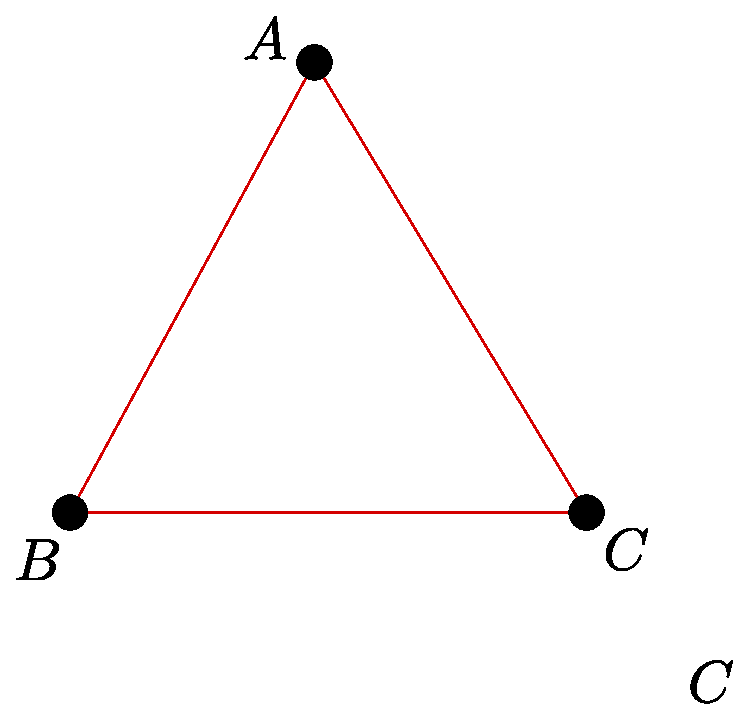
\includegraphics[scale=0.5]{Figures/Chapter1/incidence_3.eps}
                 \caption{The incidence geometry on $3$ points.}
                 \label{fig_1.1}
             \end{figure}
    \end{enumerate}
\end{example}

\begin{definition}
    In any incidence geometry, we call two lines \textbf{parellel} if they
    contain no points in commonm, or they are equal.
\end{definition}

\begin{example}\label{1.2}
    \begin{figure}[h]
        \centering
        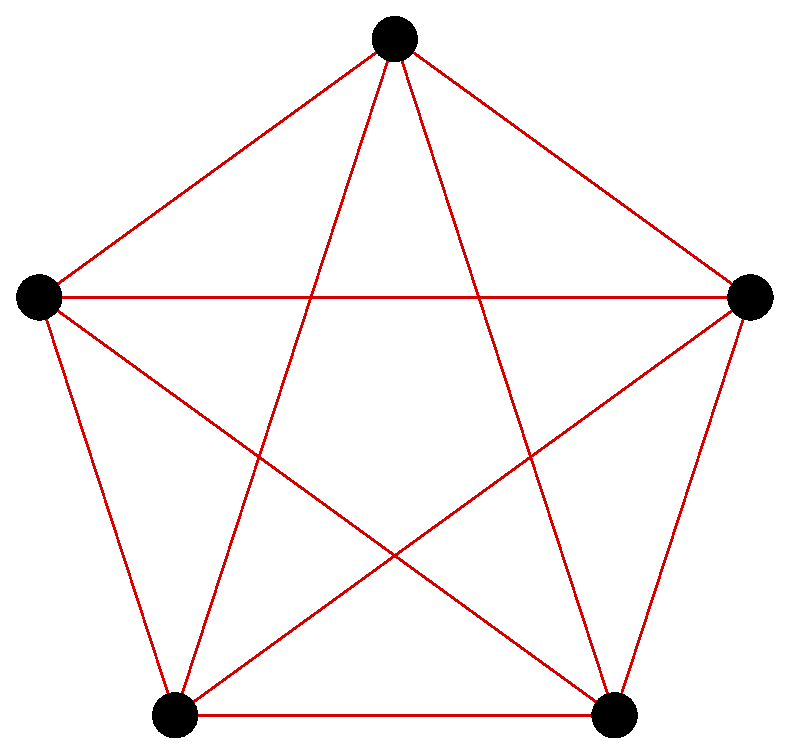
\includegraphics[scale=0.5]{Figures/Chapter1/incidence_5.eps}
        \caption{An incidence geometry on $5$ points.}
        \label{fig_1.2}
    \end{figure}
    The following figure \ref{fig_1.2} shows an incidence geometry on $5$
    points, and in which there exists parallel lines. Note that the following
    proposition is not satisfied in this geometry.
\end{example}

We have the following proposition which we accept without proof.

\begin{proposition}[Pla_yfair's Axiom]\label{1.1.2}
    For each point $A$ in an incidence geometry,  and a line $l$, there is at
    most one line passing through  $A$ and parallel to  $l$.
\end{proposition}

\begin{definition}
    Let $G$ and  $H$ be incidence geometries. We say that  $G$ and  $H$ are
     \textbf{isomorphic} if there exists a $1-1$ map  $\phi:G \rightarrow H$ of
     $G$ onto  $H$ such that if $l$ is a line in  $G$, then  $\phi(l)$ is a line
     in $H$. We call $\phi$ an \textbf{isomorphism} and we write $G \simeq H$.
     If $H=G$, then we say that $\phi$ defines an \textbf{automorphism}.
\end{definition}

\begin{proposition}\label{1.1.3}
    The axioms (I1), (I2), (I3), and Playfair's axiom are all independent of one
    another.
\end{proposition}
\begin{proof}
    Example \ref{1.2} describes a geometry in where the incidence axioms are
    satisfied, but Playfair's axiom is not.

    Alternatively, taking a two element set $G=\{A,B\}$ with its set of lines
    being $G$ satifies  (I1), (I2), and Playfair's axiom, but not (I3).

    For a geomtry satisfiying (I1), (I3) and Playfair's axiom take the geometry
    of example \ref{1.1}(2) with a line passing through the point $A$.

    Finally for a geometry satisfying (I2), (I3), and Playfair's axiom, take
    $G=\{A,B,C\}$ with collection of lines the emptyset $\emptyset$.
\end{proof}
